\documentclass{homework}

\title{Homework 3}
\author{Kevin Evans}
\studentid{11571810}
\date{February 9, 2021}
\setclass{Physics}{461}
\usepackage{amssymb}
\usepackage{mathtools}

\usepackage{amsthm}
\usepackage{amsmath}
\usepackage{slashed}
\usepackage{relsize}
\usepackage{threeparttable}
\usepackage{float}
\usepackage{booktabs}
\usepackage{boldline}
\usepackage{changepage}
\usepackage{physics}
\usepackage[inter-unit-product =\cdot]{siunitx}
\usepackage{setspace}

\usepackage[makeroom]{cancel}
%\usepackage{pgfplots}

\usepackage{enumitem}
\usepackage{times}

\usepackage{amsthm}
\newtheorem*{ident}{Identity}

\renewcommand\qedsymbol{$\blacksquare$}

\usepackage{mhchem}


\begin{document}
	\maketitle
	\begin{enumerate}
		\item \begin{enumerate}
			\item Equating its potential to the electron's rest mass, \begin{align*}
				\frac{e^2}{4 \pi \epsilon_0 r_c} & = mc^2 \\
				r_c & = \SI{2.84e-15}{m}
			\end{align*}				
		
			\item For a spin of $1/2$, we can equate its angular momentum to the classical definition as \begin{align*}
				S^2 & = \hbar^2 s (s + 1) = (mvr)^2 \\
				v^2 & = \frac{3\hbar^2 }{4 {m_e}^2 {r_c}^2} \\
					& = \frac{3 \left(\SI{1.054e-34}{\J\s}\right)^2 }{4 \left(\SI{9.11e-31}{\kg}\right)^2 \left(\SI{2.84e-15}{\kg}\right)^2} \\
					& = \SI{1.24e21}{\m\per\s}
			\end{align*}
			It's roughly 100 times $c$, which doesn't make sense.
		\end{enumerate}

		\item \begin{enumerate}
			\item The $\ell=2$ exceeds the maximum for $n=2$.
			\item The $m_\ell=2$ exceeds the maximum for $l=1$.
			\item The spin $m_s$ can only be $\pm 1/2$.
			\item Can't have a negative $\ell$ value.
		\end{enumerate}
	
		\item Since we're only looking at the valance electrons, the number of lines is determined by unpaired spins \begin{enumerate}
			\item $2$, as it's basically an H atom.
			\item $1$ as the $s$ orbital is filled.
			\item $5$ since the $p$ orbital is partially filled and there is only one paired. This means $j=1 + \frac{1}{2} + \frac{1}{2} = 2$, and it would have five lines.
			\item $5$ for the same reasoning as (c).
		\end{enumerate}
		
		\item \begin{enumerate}
			\item[(a, b)] % TODO: \usepackage{graphicx} required
			~ \\
				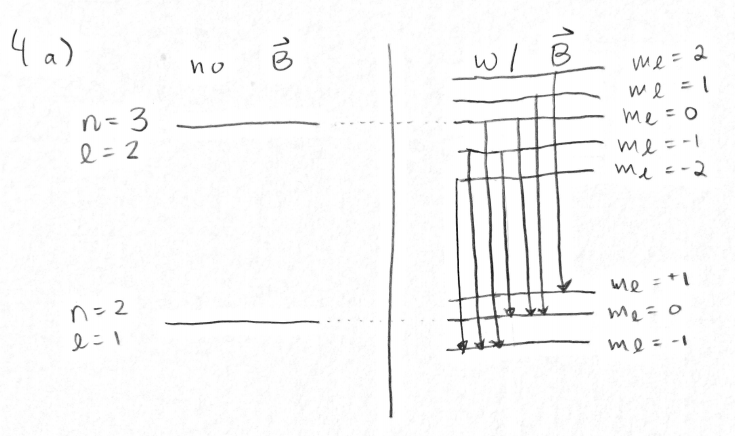
\includegraphics[width=0.7\linewidth]{hw3_1}
			\item[(c)] As $m_\ell = 0$ or $m_\ell = \pm 1$, the allowable energies are either $\Delta E=0$ or $\Delta E = \pm \mu_B \Delta m B$
		\end{enumerate}
	
		\item Between $n=3$ and $n=2$, the 
		
		\begin{enumerate}
			\item Without a magnetic field, the energy between the $n=3\to 2$ transition is \begin{align*}
				E_{3 \to 2} & = -\SI{13.6}{\eV} \left(3^{-1} - 2^{-1}\right) = \SI{1.9}{\eV}
				\intertext{Since the selection rules dictate $m_l = 0, \pm 1$, }
				\lambda & = \frac{hc}{E \pm \mu_B B m_l} \\
					& = \SI{0.197}{\eV  \um} \times \frac{1}{\SI{1.9}{\eV} \pm \SI{5.78e-5}{\eV/\tesla} \times \SI{3.5}{\tesla} \times m_l} \\
					& = \SI{103.68}{\nm}, \SI{103.67}{\nm}, \SI{103.70}{\nm}
			\end{align*}
			\item The same as (a)?
%		Here, do I just use the Rydberg constant and energy for $E_0$? $\Delta n^2 = n_2^2 - n_1^2?$
		\end{enumerate}
	
		\item \begin{enumerate}
			\item For $n=4$, \begin{itemize}
				\item $l=0$: \ce{4S_{1/2}}
				\item $l=1$: \ce{4P_{1/2}}, \ce{4P_{3/2}}
				\item $l=2$: \ce{4D_{3/2}}, \ce{4S_{5/2}}
				\item $l=3$, \ce{4F_{5/2}}, \ce{4F_{7/2}}
			\end{itemize}
		
			\item $2$ for each level?
		\end{enumerate}
	
		\item \begin{enumerate}
			\item $j=\frac{3}{2}, \frac{5}{2}$
			\item $\abs{J} = \hbar \sqrt{j(j+1)} = \frac{\hbar \sqrt{15}}{2}$, $\frac{\hbar \sqrt{35}}{2}$
			\item $J_z = \begin{cases}
				\left\{ -\frac{3\hbar}{2}, -\frac{\hbar}{2}, \frac{\hbar}{2}, \frac{3\hbar}{2} \right\} & j = \frac{3}{2} \\
				\left\{ -\frac{5\hbar}{2}, -\frac{3\hbar}{2}, -\frac{\hbar}{2}, \frac{\hbar}{2}, \frac{3\hbar}{2}, \frac{5\hbar}{2} \right\} & j = \frac{5}{2} \\
			\end{cases}$
		\end{enumerate}
	
		\item \begin{enumerate}
			\item $\ell = 2, 1, 0$
			\item $s = 1, 0$
			\item $j = 3, 2, 1, 0$
			\item $j_1, j_2 = \frac{3}{2}, \frac{1}{2}$
			\item $j = j_1 + j_2, \dots, \abs{j_1 - j_2} = 3, 2, 1, 0$. It's the same as (c)
		\end{enumerate}
	
		\item \begin{enumerate}
			\item For \SI{589.0}{\nm} and \SI{589.6}{\nm}, \begin{align*}
				E_{1/2} & = \frac{\SI{1240}{\eV \nm}}{\SI{589.6}{\nm}} = \SI{2.103}{\eV} \\
				E_{3/2} & = \frac{\SI{1240}{\eV \nm}}{\SI{589.0}{\nm}} = \SI{2.105}{\eV}
			\end{align*}
			\item $\Delta E = \SI{0.00214}{\eV}$ (or is it half of this?)
			\item The strength of the magnetic field is \begin{align*}
				\Delta E & = 2 \mu_B B \\
				B & = \frac{\Delta E}{2 \mu_B }\\
					& = \frac{\SI{0.00214}{\eV}}{2 \times \SI{5.788e-5}{\eV \per \tesla}} \\
					& = \SI{18.51}{\tesla}
			\end{align*}
		\end{enumerate}
	
		\item \begin{enumerate}
			\item As there is 9 peaks, we can use $2f + 1 = 9$, leading to a total spin of $f=4$. The lower energy level would result in $f=3$. Since $s = 1/2$, the nuclear spin must be $i=7/2$.
			
			\item Energy is added to drive the $m_j$ to their maximum/minimum state. This can be done by laser light incident on the Cesium beam.
		\end{enumerate}
	
	\end{enumerate}
\end{document}